% UTF-8

\documentclass[../main/thesis.tex]{subfiles}
\onlyinsubfile{\setcounter{chapter}{1}}  % single-chapter command
\begin{document}


\chapter{Analyse der Ausgangslage}

\begin{draft}
\section{OpenStreetMap: Alles für Alle \emph{[Entwurf]}}
Topographische Vermessungen führten ursprünglich nur zu relativ ungenauen Ergebnissen. \cf[43]{Koh04}
Für die im 18.~und 19.~Jahrhundert erstmals durchgeführte systematische Landesaufnahme standen nur am Boden operierte Messinstrumente zur Verfügung.
Bis in die zweite Hälfte des 20. Jahrhunderts waren der manuell horizontierte und abgelesene Theodolit und das Bandmaß die dabei primär eingesetzten Instrumente. \cf[3–6]{WG06}
Deren Natur entsprechend ging dies mit einem immensen Aufwand an Arbeitskräften einher.

Die schiere Menge der eingesetzten Vermesser machte im Laufe der Zeit auch mit einfachen Instrumenten zufriedenstellende Ergebnisse möglich.
In den letzten Jahrzehnten haben Photogrammetrie, Fernerkundung und satellitengestützte Ortsbestimmung das Vermessungswesen revolutioniert.
Genauere Resultate ließen sich in kürzerer Zeit und so auch mit geringeren Kosten erreichen. \noref

% Ist die Kostendiskussion wirklich von Interesse? Eigentlich geht's ja nur um die ursprüngliche Motivation für OSM

Obgleich die Kosten geringer als zuvor sind, liegen sie nach wie vor in mehrstelliger Millionenhöhe allein für die amtlichen Geobasisdaten eines deutschen Bundeslandes. \cf[3]{lgm05}
% [lgm05 3 (LG München, Beschl. vom 9. Nov. 2005, Az. 21 O 7402/02, 3; in: GRUR 2006, 225)]
In Europa \noref herrscht heutzutage \cf[119]{Fis01} die Auffassung vor, dass diese solcherart mit Steuergeldern erhobenen Daten der Allgemeinheit nicht kostfrei zur Weiternutzung zur Verfügung gestellt werden, sondern die \emph{konkreten} Nutzenden zusätzlich Lizenzgebühren zahlen sollen \noref.
Diese Lizenzkosten schränken den Nutzen amtlicher Geodaten nicht nur für kommerzielle Zwecke \cf[336]{Böh07}, sondern auch für Privatleute \noref erheblich ein \noref.

% [Egg99 \noref]

Heute haben selbst billige GPS-Empfänger eine Genauigkeit, welche die mancher Vermessung des 19. Jahrhunderts übertreffen kann. \cf[346][\?]{WG06}
Die „freie Weltkarte“ \eyecatcher{OpenStreetMap} (OSM) \cf[3]{RT09} macht sich dies zu Nutze, um mit Hilfe zehntausender Freiwilliger eine weltweite Datenbank mit Geobasisdaten aufzubauen und nachzuführen (Volunteered Geographic Information, VGI). \cf[147, 154]{NZ12}
Im Gegensatz zu vielen amtlichen Geobasisdaten dürfen OpenStreetMap-Daten lizenzkostenfrei verwendet werden, auch für kommerzielle Zwecke. \cf[217, 221\f]{RT09}

% ODBL? -> 3rd ed

% fühlt sich alles _viel_ zu lang an … was davon brauche ich wirklich als Überleitung zu Fragmentierung und Process?
% straff kürzen, unbekannte Begriffe a la KV-Pair einfach in Fußnote packen…
% Oder wild ausdehnen, z. B. Verweis auf NoSQL-Prinzip hinsichtlich Flexibilität? … Nein, das ist nicht Aufagbe dieser Arbeit. Lieber noch mehr Verweise suchen.

Der Name OpenStreetMap mag fehlleitend sein, denn es handelt sich dabei nicht um eine Straßenkarte, sondern vielmehr um eine Geodatenbank mit Inhalten nahezu beliebiger Themen.
Bei der Gründung von OSM im Jahr 2004 wurde auf das Festlegen starrer Klassifizierungsschemata oder Kartierschlüssel verzichtet.
Statt dessen kann jedes Element in der Datenbank mit einer beliebigen Anzahl Attribute – sogenannter \term{tags} – versehen werden, die jeweils aus einem Schlüssel und einem Wert bestehen \term{(key-value-pair)}. \cf[56]{RT09}

% ways / relationen / fragmentierung !!

Syntax und Semantik der einzelnen \term{tags} werden bei OpenStreetMap seit der Gründung fortlaufend von den Beitragenden diskutiert, gestützt auf bisherige Erfahrungen.
Die Diskussion findet vornehmlich im Internet statt; Ergebnisse werden öffentlich dokumentiert und in Software wie z.~B. Renderern implementiert.
Wer neue Inhalte erfasst, orientiert sich oft an den bisher in der Datenbank üblichen oder im Web dokumentierten Konventionen. \cf[48]{Top09} \cf[17\f, 59–66]{RT09}

Gegenüber einer vor der Erfassung vereinbarten gemeinsamen Ontologie \cf[14]{GOS09} hat dieses System zur Folge, dass die zu OSM Beitragenden genau das erfassen, was sie persönlich interessiert und für wichtig halten.
Jeder der Beitragenden entscheidet die Kriterien für die Erfassungsgeneralisierung für sich selbst.
%Dies führt zu großen regionalen Unterschieden in Datendichte, -aktualität und -qualität.
% Regionalität ist nicht entscheidend für uns.

% Verweis auf Sch09 deckt schon vieles ab; Kne09 eher knapp, Beh11 noch knapper, Kla11 umständlich

\label{osm-fragmentation}

Oft verfügen die OpenStreetMap-Daten über sehr hohen Detailreichtum.
So könnten zum Beispiel für Teilstücke einer Straße \term{tags} für Tempolimits, Überholverbote, Fahrspurenanzahl, Oberflächenmaterial sowie -Qualität, Baujahr und mehr eingetragen worden sein.
Veränderungen an diesen Attributen im Verlauf der Straße führen im OSM-Datenmodell zwangsläufig zu einer Fragmentierung in mehrere aufeinander folgende Linienabschnitte \term{(ways)}, jeweils mit unterschiedlichen \term{tags}. \cf[57]{RT09}

% "Detailreichtum entsprechend einer Grundkarte" (?) -> verdeutlicht, dass OSM ungeneralisiert ist

Baulich getrennte Fahrbahnen wie etwa Autobahnen bildet OpenStreetMap mittels zweier paralleler Einbahn-Linienzüge ab. \cf[62]{RT09}
Dies ist eine in der Geoinformatik gängige Vorgehensweise. \cf[2][\?]{Tho05}

Sowohl die Fragmentierung als auch die parallelen Linienzüge führen zu Schwierigkeiten in der Weiterverarbeitung und Visualisierung. \noref[Mig12 u. a.]
% Abbildungen:
% - Marker-Wucherung
% - stark unregelmäßige Plazierung von Namen \cf{Mig12}
% - Blitzer/Freistellung
% - Doppelnamen \cf{Mig12}
% o. ä.
Offensichtlich ist, dass eine Verkettung der Fragmente bzw. parallelen Linienzüge als Bestandteil des Datenmodells die Probleme wesentlich verkleinern, wenn nicht gar gänzlich lösen würde.
Für eine hierarchisch orientierte Organisation wie etwa Vermessungsämter wäre eine solche Lösung naheliegend.
Über \term{relations} ist dies auch in OpenStreetMap möglich. \cf[57]{RT09}
Das oben beschriebene Fehlen interner Strukturen unter den zu OpenStreetMap Beitragenden (der \term{community}) macht es jedoch unmöglich, „mal eben“ die Regeln für die Erfassung und Kodierung der Geodaten zu ändern. \cf{Sch09}

% unklar: "hierarchisch orientierte Organisation"? gemeint ist wohl das Ding mit der manuell gepflegten Mittellinie in den Daten?

Statt dessen müssen Änderungsvorschläge erst von der \term{community} akzeptiert und anschließend \emph{großräumig} und \emph{korrekt} in der Datenbank Anwendung finden.
Die Erfahrung zeigt, dass dies ein langwieriger Prozess sein kann, der umso schwieriger wird, je geringer der unmittelbare Einfluss der Datenbank-Änderungen auf das in Karten sichtbare Ergebnis ist \noref.


% OSM ist per design völlig ungeneralisiert, da maßstabslos und für auch sehr große maßstäbe eingesetzt. WIrd das im Zusammenhang deutlich? wichtig für logik im folgeabschnitt
\end{draft}



%\biggap

\section{Kartenherstellung mit OpenStreetMap} \label{kartenherstellung}

Wohl am bekanntesten ist OpenStreetMap für die auf der Projekt-Homepage \href{https://www.openstreetmap.org/}{\nolinkurl{osm.org}} zugängliche Web-Karte (Abbildung~\ref{fig:osm.org}).
Sie besteht aus quadratischen Kacheln \term{(tiles)} von $256\times\unit[256]{px}$, die dort in 19 verschiedenen Maßstäben%
\footnote{In 2013 wurde ein noch größerer, 20.~Maßstab ergänzt (bei null beginnend gezählt \cf{Dijk82} die Zoomstufe~19).}
angeboten werden von etwa $1 \nobreak : \nobreak 2000$ bis $1 \nobreak : \nobreak 500~\unit{Mio.}$ \cf[154–155]{RT09}
Eine interaktive Oberfläche erlaubt über die freie Wahl der Zoomstufe eine Maßstabswahl und macht den Kartenausschnitt verschiebbar, so dass jeder im eingesetzten Kartennetz abbildbare Punkt der Erde angezeigt werden kann.
% evtl. Datenmenge etc. betonen

\onefigure{ht}{
	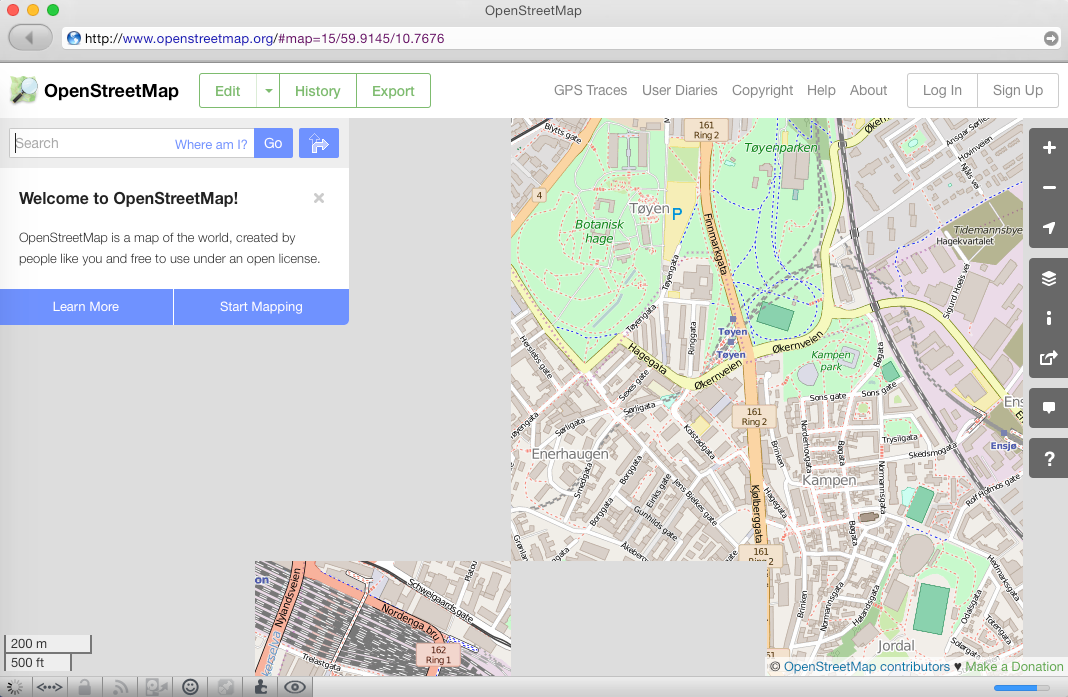
\includegraphics[width=\ScaleIfNeeded]{../chapter2/osm-org}
	\caption{Projekt-Homepage von OpenStreetMap während des Ladevorgangs}
	\label{fig:osm.org}
}

Wegen der sehr großen Anzahl von Kacheln werden diese in größeren Maßstäben \term{just in time} gezeichnet. \cf{osm:TileUsage}
Die Kartenbasis ist für alle Maßstäbe die jeweils minutengenau aktualisierte OSM-Datenbank.
%\noref % TODO: evtl. Verweis auf RT09, insb. für basis, minutengenau -> p. 157 zu osmarender, -> p. 195 zu diffs

Diese schnelle Aktualisierung ist für OpenStreetMap besonders wichtig, um den freiwillig Mitwirkenden nach einem Beitrag zur Datenbank ein schnelles Erfolgserlebnis zu geben, indem der Beitrag in der Karte weltweit für jeden sofort sichtbar wird.
Aus diesem Grund muss jede Generalisierung der Karte automatisiert ablaufen.
Weiterhin bedeutet die Zahl der Beiträge mit teilweise über 1000 \term{changesets} pro Stunde, \cf{Nei15}
% http://osmstats.neis-one.org/?item=changesets&date=7-11-2015
% http://neis-one.org/2013/08/osm-activity-report-2013/
dass der Arbeitsaufwand für eine manuelle Generalisierung prohibitiv hoch wäre.
Klassische kartographische Generalisierung von Hand kommt daher nur für nicht nachzuführende und geographisch begrenzte Einzelanfertigungen in Betracht, etwa wenn auf Basis von OpenStreetMap eine traditionelle gedruckte Karte hergestellt werden soll.

Typischerweise besteht die Grundlage für Web-Karten wie derjenigen auf \url{osm.org} aus einer Geodatenbank, die mit einer Kopie der OpenStreetMap-Datenbank gefüllt und anschließend minütlich aktualisiert wird (Abbildung~\ref{fig:osm-datenfluss}).
Diese Geodatenbank enthält die Geometrie und Attribute \term{(tags)} der Rohdaten.
Vom Kartenleser in der interaktiven Oberfläche im Webbrowser erzeugte Anfragen nach Kacheln der Karte werden dann von der Renderer-Software unter Zugriff auf die Geodatenbank abgearbeitet, wobei die Geometrie anhand der vorgegebenen Zeichenregeln dargestellt wird.
Gerenderte Kacheln werden in einem Cache abgelegt und zum Browser geschickt.

Eigene Bearbeitungsschritte zur Generalisierung von Daten sind bei diesem Ablauf nicht vorgesehen (im Gegensatz zu den Abläufen im AAA-Modell der deutschen Landesvermessung \cf[263]{ML12}).
Lediglich als Nebeneffekt des Einlesens in die Datenbank und des Zeichnens durch den Renderer wird eine begrenzte Modell-\noncf[194 17.2]{RT09} bzw. kartographische Generalisierung durchgeführt. \cf[194, 198]{RT09}
% [ML12] beschreibt einzelne kommerzielle Lösung (hat aber nette Bilder); -> möglichst noch bessere Quelle suchen
% http://wiki.openstreetmap.org/wiki/Mod_tile/Setup_of_your_own_tile_server

\onefigure{ht}{
	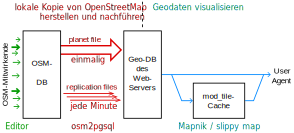
\includegraphics[width=\ScaleIfNeeded]{../chapter2/osm-datenfluss}
	\caption{typischer \osm-Datenfluss (vereinfacht dargestellt)}
	\label{fig:osm-datenfluss}
	% Mapnik nur ein Beispiel
}


% obiges trifft auf Linien, Punkte, Flächen gleichermaßen zu; hier darauf eingehen?


% LVAs verwenden (?) kartographische Hints, um die Ableitung von FOlge-DLMs zu erleichtern (?) [ML12, KN 62 (5) 263]. Das geht bei OSM nicht, weil auch das eben die Generalisierung und damit auch die Kartenherstellung verzögern und somit das schnelle ERfolgserlebnis verhindern würde. Es muss eben tatsächlich vollautomatisch ablaufen, wie auch immer.

% lesen: -> KN 56 (4) 191ff Modellgeneralisierung in ATKIS


% MapCSS includes an eval function, and has rules that act as 'commands' to modify data. CartoCSS does not support eval or any data-modifying operations.
% https://gist.github.com/tmcw/4319642


% Angesichts dessen wären automatisiert abgeleitete, generalisierte Datenbanken für kleinere Maßstäbe zur Weiterverwendung wünschenswert, existieren jedoch bisher nicht. Entsprechend sind auch die aus OSM-Daten hergestellten Karten in aller Regel nicht kartographisch generalisiert: Nahe beieinander liegende Objekte überdecken einander scheinbar wahllos, Mindestgrößen und notwendige Formvereinfachungen werden von den automatischen Renderern ignoriert.

% Erschwert wird die Generalisierung von OSM-Daten unter anderem durch den hohen Grad der Fragmentierung von Linienzügen. Das Verknüpfen solcher zusammengehörenden, einzelnen ways durch Relationen in der Datenbank ist technisch möglich, wird aber von den Mitwirkenden aus unterschiedlichen Gründen nur sehr selten durchgeführt. Eine automatisierte Generalisierung durch Formvereinfachung (zur Reduktion der node-Anzahl) bedingt daher, dass die zusammengehörenden ways  dabei  als solche identifiziert werden. Gleiches gilt für die Generalisierung durch Zusammenfassung oder Verdrängung parallel verlaufender Linienzüge, beispielsweise Straßen mit begleitendem Radweg oder mehrgleisigen Bahnstrecken.



\section{Automatisierte Linien-Generalisierung von OpenStreetMap-Daten}

Wie im Folgenden einige Beispiele zeigen, lassen sich von den sieben elementaren Generalisierungsvorgängen \cf[168]{HGM02} die Auswahl auf Basis der Objektklasse sowie die Betonung und Vergrößerung durch veränderte Strichbreite vergleichsweise einfach im Renderer implementieren, da die Geometrie der zugrundeliegenden Geodaten dabei unverändert bleibt.
Andere Arten kartographischer Generalisierung wie etwa die Formvereinfachung oder der Qualitätsumschlag würden die Geometrie verändern, sind damit schwieriger zu implementieren und werden bisher nicht oder kaum eingesetzt.



\subsection{Generalisierung durch Objektauswahl}

Zur Herstellung der Kacheln der Web-Karte wird für jede Zoomstufe eine Auswahl der jeweils darzustellenden Objektklassen vorgenommen.
Beispielsweise werden Anliegerstraßen \term{(residentials)} unterhalb von Zoom~12 nicht mehr dargestellt (Abbildungen~\ref{fig:kampen11} und~\ref{fig:kampen12}).
Dies vereinfacht das Kartenbild für den Betrachter und verringert die zu berechnende Datenmenge für den Renderer.

% Qualitätsumschlag fällt in OSM tlws. auch hierunter, gibt's aber nur für Flächen

\twofigures{t}{
	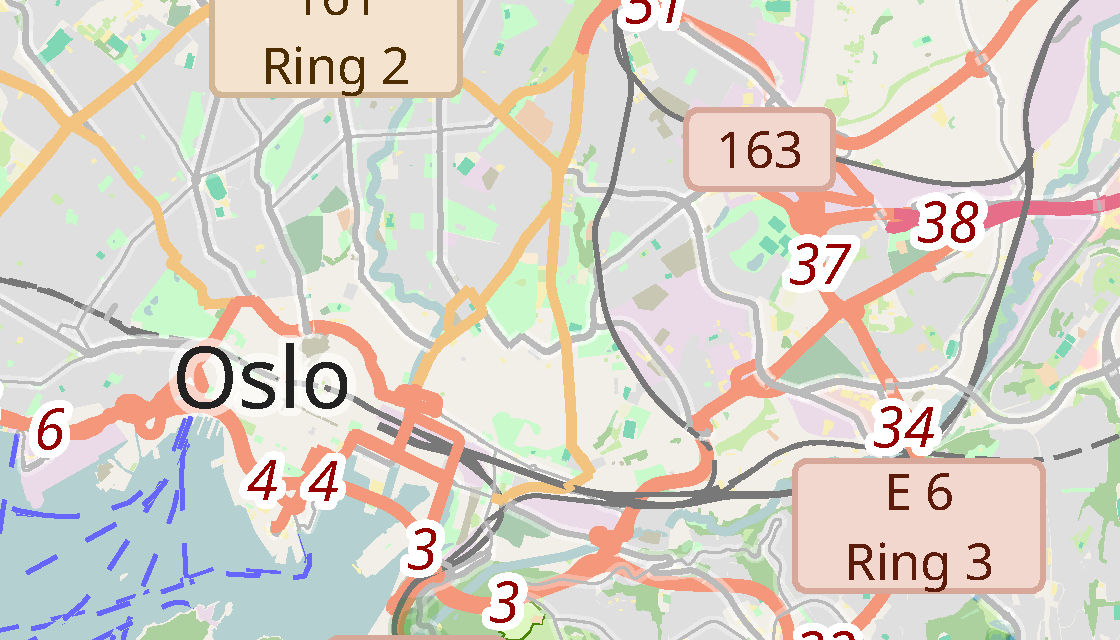
\includegraphics[width=\ScaleIfNeeded]{../chapter2/kampen-z11}
	\caption
		[Karte von \nolinkurl{osm.org}, Zoom~11, \term{residentials} nicht dargestellt]
		{Karte von \nolinkurl{osm.org}, Zoom~11, \term{residentials} nicht dargestellt \citex{map:osm-carto}}
	\label{fig:kampen11}
}{
	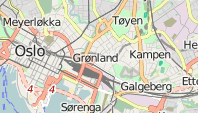
\includegraphics[width=\ScaleIfNeeded]{../chapter2/kampen-z12}
	\caption
		[Karte von \nolinkurl{osm.org}, Zoom~12, \term{residentials} dargestellt]
		{Karte von \nolinkurl{osm.org}, Zoom~12, \term{residentials} dargestellt \citex{map:osm-carto}}
	\label{fig:kampen12}
}



\subsection{Generalisierung durch Vergrößerung}
% Vergrößerung -> maßstabsbedingt notwendig

\twofigures{t}{
	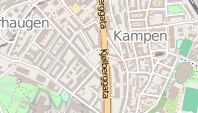
\includegraphics[width=\ScaleIfNeeded]{../chapter2/kampen-z14}
	\caption
		[Karte von \nolinkurl{osm.org}, Zoom~14, \term{residentials} 3~Pixel breit]
		{Karte von \nolinkurl{osm.org}, Zoom~14, \term{residentials} $\unit[3]{px}$ breit \citex{map:osm-carto}}
	\label{fig:kampen14}
}{
	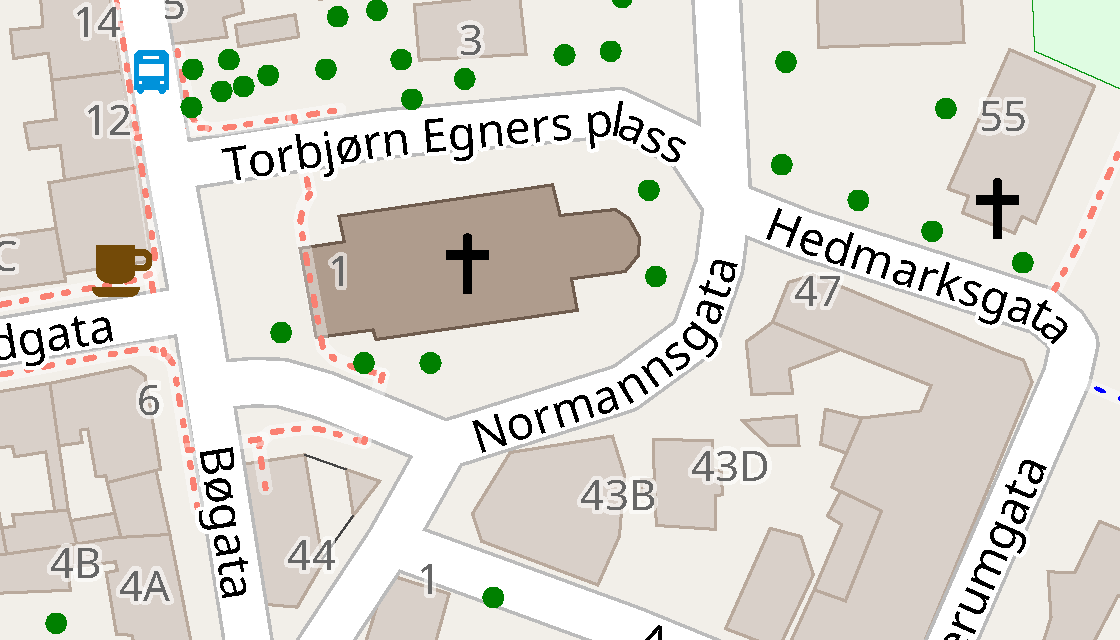
\includegraphics[width=7cm]{../chapter2/kampen-z17}
	\caption
		[Karte von \nolinkurl{osm.org}, Zoom~17, \term{residentials} 12~Pixel breit]
		{Karte von \nolinkurl{osm.org}, Zoom~17, \term{residentials} $\unit[12]{px}$ breit \citex{map:osm-carto}}
	\label{fig:kampen17}
}

\capstartfalse  % empty figures aren't supported by the document class
\twofigures{t!}{
	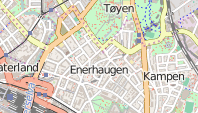
\includegraphics[width=\ScaleIfNeeded]{../chapter2/kampen-z13}
	\caption
		[Karte von \nolinkurl{osm.org}, Zoom~13, \term{residentials} 3~Pixel breit]
		{Karte von \nolinkurl{osm.org}, Zoom~13, \term{residentials} $\unit[3]{px}$ breit \citex{map:osm-carto}}
	\label{fig:kampen13}
}{
}
\capstarttrue

Die Wahl der Zeichenregeln beinhaltet für einige Objektklassen auch eine Generalisierung durch Vergrößerung, indem für bestimmte Maßstäbe eine Strichbreite gewählt wird, welche im Abbildungsmaßstab die tatsächliche Größe des Objekts übersteigt.
Anliegerstraßen haben für die Zoomstufen 14 bis~19 jeweils eine unterschiedliche Strichbreite von $\unit[3]{px}$ bis $\unit[17]{px}$ definiert, so dass die Darstellung der Straße in der Karte Maßstabsänderungen andeutungsweise folgt (Abbildungen~\ref{fig:kampen14} und~\ref{fig:kampen17}). \cf{All15}
Die Breite von $\unit[3]{px}$ auf \term{zoom} 14 entspräche ca.~$\unit[27]{m}$ in der Realität. \cf[155]{RT09}
Auf \term{zoom} 13 werden Anliegerstraßen gar auf dieselbe Breite von $\unit[3]{px}$ gezeichnet (ca.~$\unit[57]{m}$) und damit deutlich vergrößert, um die Erkennbarkeit im kleinerem Maßstab zu fördern (Abbildungen~\ref{fig:kampen14} und~\ref{fig:kampen13}).

% z13+z14 erst 2015 exakt gleiche Strichbreite:
% https://github.com/gravitystorm/openstreetmap-carto/blob/fe4f8d48757cf85bb692129b5d9755ba5cadbbee/roads.mss
%@residential-width-z13:           3;
%@residential-width-z14:           3;
%@residential-width-z15:           5;
%@residential-width-z16:           6;
%@residential-width-z17:          12;
%@residential-width-z18:          14;
%@residential-width-z19:          21;



\subsection{Generalisierung durch Bewertung}
% Bewertung -> nach Bedeutung für den Kartenzweck

Weiterhin wird durch die Wahl der Zeichenregeln eine Bewertung der tatsächlich dargestellten Objekte vorgenommen, auch dies abhängig vom Maßstab.
So werden Anliegerstraßen auf \term{zoom}~12 als schmaler, einfacher Strich gezeichnet, ab \term{zoom}~13 jedoch als weißer Breitstrich mit grauem Rand (Abbildungen~\ref{fig:kampen12} und~\ref{fig:kampen13}).

% weitere Fälle von Bewertung: evtl. Klassifizierung nach primary, secondary etc mit unterschiedlich definierten Strichbreiten? TODO: verifizieren

%Ein unklares Kartenbild ist jedoch auch in weniger exotischen
% "näher liegenden"?
%Konstellationen zu beobachten. Ein weit verbreitetes Problem ist beispielsweise
%In vielen Fällen lässt sich allerdings ein unklares Kartenbild

\label{dual-highway-case-1}

Ein weit verbreitetes unklares Kartenbild lässt sich allerdings als scheinbare Betonung einiger auf \url{osm.org} gezeichneten Straßen missverstehen, wie Abbildung~\ref{fig:utrecht14} beispielhaft zeigt.
Die als Sammelstraße klassifizierte Croeselaan (bei Markierung~\textfiguremark{1}) wird mit breiterem Strich gezeichnet als Teile der Hauptstraßen (bei~\textfiguremark{2}).
Grund dafür sind nicht tatsächliche Unterschiede im Ausbauzustand%
\footnote{Der kürzlich begonnene in der Abbildung bei~\textfiguremark{2} zu erkennende Neubau einer Busfahrbahn verschmälert die Hauptstraße nicht.}
oder der Verkehrsbedeutung, sondern der Umstand, dass die Fahrbahnen der niederrangigen Straße durch einen breiten, parkähnlichen Grünstreifen getrennt werden  (Abbildung~\ref{fig:utrecht16}).
In kleinerem Maßstab überlappen sich die verbreitert gezeichneten Signaturen der beiden Fahrbahnen und fließen zusammen, so dass sich für den Betrachter der Eindruck einer besonders breiten oder wichtigen Straße ergibt.

Gleiches gilt für die ebenfalls in Abbildung~\ref{fig:utrecht14} auffallende wechselhafte Strichbreite einer Hauptstraße:
Hier existiert bei Markierung~\textfiguremark{2} nur eine einzige Fahrbahn, während sich bei~\textfiguremark{3} die Signaturen von zwei parallelen Fahrbahnen überlappen.

\twofigures{ht}{
	\begin{overpic}[width=\ScaleIfNeeded]{../chapter2/utrecht-z14}
		\put(115,48){\figureframe{.25}}
		\put(121,54){\figuremark[white]{1}}
		\put(30,45){\figuremark[white]{2}}
		\put(19,94){\figuremark[white]{3}}
	\end{overpic}
	% http://render.openstreetmap.org/cgi-bin/export?bbox=5.099716,52.074811,5.122461,52.082776&scale=30000&format=pdf
	\caption
		[Karte von \nolinkurl{osm.org}, Zoom~14, Zusammenfließen benachbarter Fahrbahnen]
		{Karte von \nolinkurl{osm.org}, Zoom~14, Zusammenfließen von benachbarten Fahrbahnen \citex{map:osm-carto}}
	\label{fig:utrecht14}
}{
	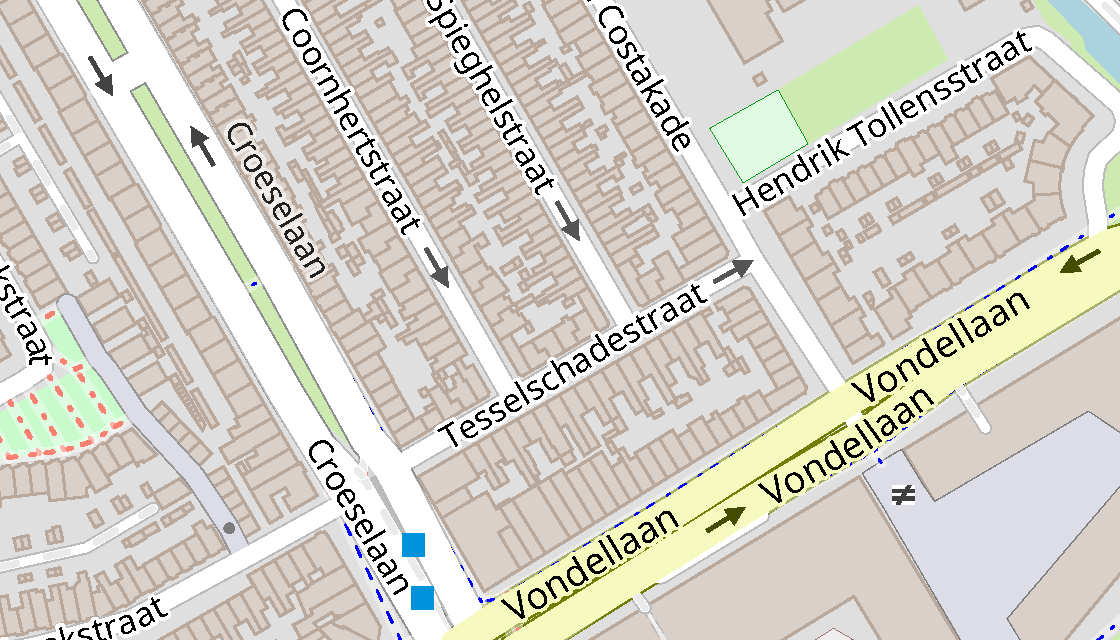
\includegraphics[width=\ScaleIfNeeded]{../chapter2/utrecht-z16}
	% http://render.openstreetmap.org/cgi-bin/export?bbox=5.112805,52.078108,5.118492,52.080099&scale=7500&format=pdf
	\caption
		[Karte von \nolinkurl{osm.org}, Zoom~16, Fahrbahnen getrennt erkennbar]
		{Karte von \nolinkurl{osm.org}, Zoom~16, Fahrbahnen getrennt erkennbar (\textfiguremark{1} in Abbildung~\ref{fig:utrecht14}) \citex{map:osm-carto}}
	\label{fig:utrecht16}
}

Abbildung~\ref{fig:gera13} zeigt ein ähnlich unklares Kartenbild.
Hier ist die Hauptstraße längs der Eisenbahnstrecke bei Markierung~\textfiguremark{1} deutlich breiter als bei \textfiguremark{2}.
Auch hier liegt keine gezielte Bewertung vor; vielmehr wird die Straße von der Bahnstrecke teilweise verdeckt, so dass die Karte den falschen Eindruck einer unterschiedlichen Strichbreite verschafft.

\twofigures{ht}{
	\begin{overpic}[width=\ScaleIfNeeded]{../chapter2/gera-z13}
		\put(52,54){\figuremark[white]{1}}
		\put(64,77){\figuremark[white]{2}}
%		\put(23,44){\figureframe{.5}}
%		\put(118,96){\figuremark[white]{3}}
	\end{overpic}
	% http://render.openstreetmap.org/cgi-bin/export?bbox=12.058353,50.868971,12.102371,50.884842&scale=70000&format=pdf
	\caption
		[Karte von \nolinkurl{osm.org}, Zoom~13, Straße teilweise durch Bahnstrecke verdeckt]
		{Karte von \nolinkurl{osm.org}, Zoom~13, Straße teilweise durch Bahnstrecke verdeckt \citex{map:osm-carto}}
	\label{fig:gera13}
}{
	\begin{overpic}[width=\ScaleIfNeeded]{../chapter2/gera-z14}
		\put(65,21){\figuremark[white]{1}}
		\put(82,57){\figuremark[white]{2}}
	\end{overpic}
	% http://render.openstreetmap.org/cgi-bin/export?bbox=12.063503,50.875014,12.085512,50.88295&scale=35000&format=pdf
	\caption
		[Karte von \nolinkurl{osm.org}, Zoom~14, Straße neben Bahnstrecke]
		{Karte von \nolinkurl{osm.org}, Zoom~14, Straße neben Bahnstrecke \citex{map:osm-carto}}
%		{Karte von \nolinkurl{osm.org}, Zoom~14, Straße neben Bahnstrecke (\textfiguremark{3}~in Abbildung~\ref{fig:gera13}) \citex{map:osm-carto}}
	\label{fig:gera14}
}

Interessanterweise kehrt sich in größerem Maßstab das Verhältnis der Strichbreiten um:
In Abbildung~\ref{fig:gera14} ist die Hauptstraße bei Markierung~\textfiguremark{1} nun deutlich \emph{schmaler} als bei~\textfiguremark{2}.
Dies liegt an getrennt erfassten Richtungsfahrbahnen bei~\textfiguremark{2}, wie sie schon in Abbildung~\ref{fig:utrecht16} gezeigt wurden, während bei~\textfiguremark{1} mangels baulicher Trennung der beiden Fahrtrichtungen nur ein einziger Linienzug erfasst ist.
Wiederum handelt es sich nicht um eine gezielte Bewertung; der Anschein unterschiedlicher Strichbreiten ist unbeabsichtigt.

%(Dies könnte durch Verdrängung gelöst werden; siehe dort.)



\subsection{Generalisierung durch Formvereinfachung}

Eine kartographische Formvereinfachung wird für die Web-Karte nicht vorgenommen.
Zufriedenstellende voll automatisiert arbeitende Algorithmen dafür stehen nicht zur Verfügung und ein Eingreifen von Hand ist wie zuvor in Abschnitt \ref{kartenherstellung} erläutert nicht vorgesehen. \cf[25]{Kla11}
In kleineren Maßstäben ergibt dies beispielsweise für Straßen mit vielen kleineren Kurven eine zittrige Darstellung, so etwa in Abbildung~\ref{fig:trollstigen-osm} bei Markierung~\textfiguremark{1}.
Der Leser kann mit etwas Phantasie zwar erkennen, dass die Straße nicht absolut gerade verläuft, jedoch macht dies die Darstellung undeutlich und ist auch in diesem Maßstab nicht von Bedeutung.

\twofigures{ht}{
	\begin{overpic}[width=\ScaleIfNeeded]{../chapter2/trollstigen-z11}
		\put(87,16){\figuremark[white]{1}}
		\put(125,52){\figuremark[white]{2}}
	\end{overpic}
	\caption
		[Trollstigen, Web-Karte mit \osm-Daten, $1\nobreak:\nobreak135\,000$]
		{Trollstigen, Web-Karte mit \osm-Daten, $1\nobreak:\nobreak135\,000$ \citex{map:thunderforest}}
	\label{fig:trollstigen-osm}
}{
	\begin{overpic}[width=7cm]{../chapter2/trollstigen-kartverket-z11}
		\put(87,16){\figuremark[white]{1}}
		\put(125,52){\figuremark[white]{2}}
	\end{overpic}
	% replace Kartverket placeholder with custom-made example?
	% this example may be at a different scale than the OSM image!
	\caption
		[Trollstigen, manuell kartographisch generalisiert, $1\nobreak:\nobreak135\,000$]
		{Trollstigen, manuell kartographisch generalisiert, $1\nobreak:\nobreak135\,000$ \citex{map:n250}}
	\label{fig:trollstigen-manual}
}

An Serpentinen fällt dieser Mangel an Generalisierung besonders auf (Markierung~\textfiguremark{2}).
Im Extremfall kann sich hier in kleinem Maßstab durch das Zusammenfließen der Strecken zwischen den Kehren der falsche Eindruck einer großen, ebenen Straßenfläche ergeben (Abbildung~\ref{fig:trollstigen-osm}).
Eine sorgfältige Formvereinfachung müsste dagegen den Charakter der Straße durch Darstellung nur einiger ausgewählter Kehren mit vereinfachtem Verlauf erhalten (Abbildung~\ref{fig:trollstigen-manual}).
%Die Abbildungen~\ref{fig:trollstigen-osm} und~\ref{fig:trollstigen-manual} zeigen auch, wie in der kartographischen Generalisierung die Serpentinen als das Signifikante dieser Straße betont und die unwesentlichen kleineren Kurven davor und danach durch Formvereinfachung entfallen.

„Die Formvereinfachung ist insgesamt eine Reduzierung der Anzahl von Stützpunkten, wenngleich u.~U. lokal Stützpunkte hinzugefügt werden, um typische Formen übertreibend zu betonen.“ \citex[Formv.]{BK01}
Während letzteres nach Kenntnis des Verfassers gegenwärtig nicht automatisiert möglich ist, kann eine bloße Reduzierung der Zahl der Stützpunkte zur Linienglättung automatisiert erfolgen.
Ein wichtiger Nebeneffekt ist dabei die verringerte Menge an Geodaten und damit deren vereinfachte Verarbeitung.
Der vielfach benutzte Algorithmus von Ramer, Douglas und Peucker zur Linienglättung zielt gerade auf Effizienz ab („efficient representation“ \citex[244]{Ram72}).
Eine Formvereinfachung nach kartographischen Gesichtspunkten ergibt sich mit ihm in der Regel nicht.

\onefigure{!b}{
	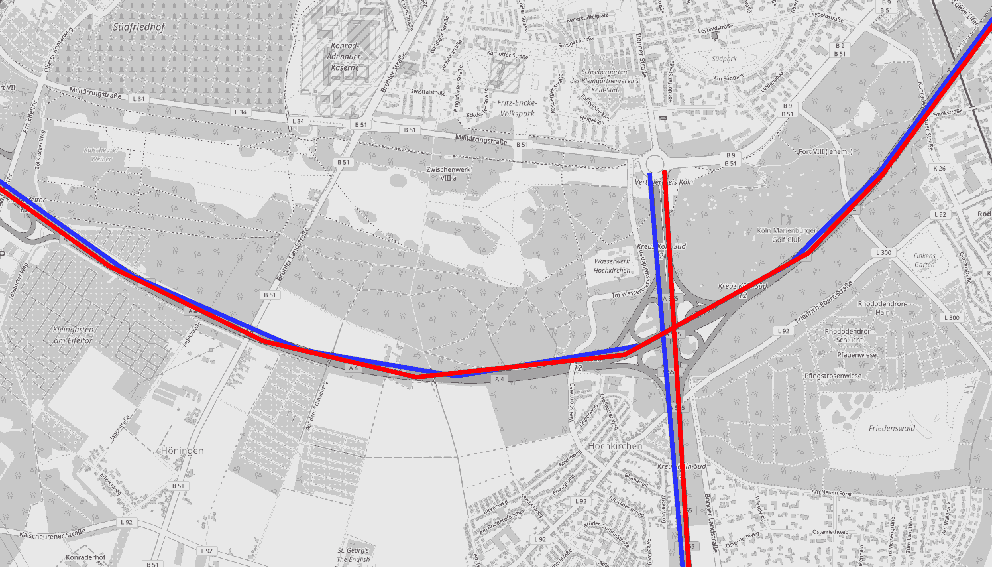
\includegraphics[width=12.25cm]{../chapter2/crossing}
	\caption
		[Überkreuzen paralleler Linienzüge nach Vereinfachung mit Ramer-Doug\-las-Peucker]
		{Überkreuzen paralleler Linienzüge nach Vereinfachung mit Ramer-Douglas-Peucker \citex[entsättigt][Hintergrund]{map:osm-carto}}
	\label{fig:crossing-parallels}
}
% TODO: Grafik neu erstellen: Originalkarte -> PSD -> Image/Adjustments/Black&White + QGIS-Export zur Registrierung => PDF in AI

Eines der Probleme bei der Automatisierung der Formvereinfachung besteht in der Notwendigkeit, alle vereinfachten Linien aufeinander abzustimmen, damit die charakteristischen Formen im Kartenbild insgesamt erhalten bleiben. \cf[\ibidabbr]{BK01}
%Formvereinfachung in kartographisch relevantem Ausmaß wäre daher nur mit einem ganzheitlichem Ansatz sinnvoll, der alle Objektklassen berücksichtigt und sie zueinander passend generalisiert.
%Beispielsweise müsste der Verlauf einer in einem engen Flusstal verlaufenden Straße in gleicher Weise vereinfacht werden wie der Verlauf des Flusses.
%Wenn nötig, müsste eines dieser beiden Objekte dazu auch verdrängt werden.
%Ein derart aufwändiger Vorgang wird nicht von dem für die Web-Karte genutzten Renderer Mapnik implementiert.
%Es wäre ein separater vorgeschalteter Schritt notwendig, welcher aus der lokalen ungeneralisierten Geodatenbank eine separate generalisierte Geodatenbank erzeugt, die dann von Mapnik gerendert werden könnte.
%Dies ist derzeit nicht der Fall.
Dies wird unter anderem dort deutlich, wo parallele Linienzüge mit Ramer-Douglas-Peucker vereinfacht werden.
%Optisch besonders auf{\nolig}fällig ist fehlende Erkennung paralleler Linienzüge als zusammengehörig, wenn sie einer starken Formvereinfachung unterzogen werden.
%Weil beide Linien dann unabhängig voneinander generalisiert werden, kann es abhängig vom eingesetzten Algorithmus zu unterschiedlichen Formen der beiden Linien kommen, die sich im Extremfall sogar gegenseitig überkreuzen können (Abbildung~\ref{fig:crossing-parallels}).

Beispielsweise zeigt Abbildung~\ref{fig:crossing-parallels} Richtungsfahrbahnen von Autobahnen, die nach Vereinfachung mit Ramer-Douglas-Peucker durch die ungleichmäßige Verteilung ihrer Stützpunkte stark variierende Abstände zueinander haben und sich sogar teilweise überkreuzen.
Dieses Problem ließe sich wenigstens für den Fall paralleler Linien leicht umgehen, wenn diese vor der Formvereinfachung zusammengefasst werden könnten.

Als weiteres Beispiel sind breite Flüsse zu nennen, für die in OpenStreetMap üblicherweise neben einer Mittellinie auch beide Uferlinien erfasst sind, um die flächenhafte Ausdehnung abzubilden.
Je nach den gewählten Parametern kann eine Formvereinfachung hier dazu führen, dass die Mittellinie das Flussbett verlässt. \cf[57]{Kla11}



\subsection{Generalisierung durch Verdrängung}

Typisch für Web-Karten ist das völlige Fehlen von Verdrängungen zur Einhaltung kartographischer Minimalabstände und -dimensionen.
Statt dessen werden mit kleiner werdendem Maßstab Objekte dichter und dichter aneinander, schließlich gar übereinander gezeichnet, worunter das Kartenbild teils erheblich leidet (Abbildung~\ref{fig:verdraengung}).
Web-Karten mit \osm-Daten sind hier keine Ausnahme.

\onefigure{ht}{
	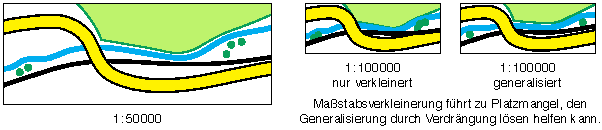
\includegraphics[width=13cm]{../chapter2/verdraengung}
	\caption
		[typisches Generalisierungsergebnis in Web-Karten]
		{typisches Generalisierungsergebnis in Web-Karten \cf[49]{sgk02}}
	\label{fig:verdraengung}
}

\twofigures{H}{
	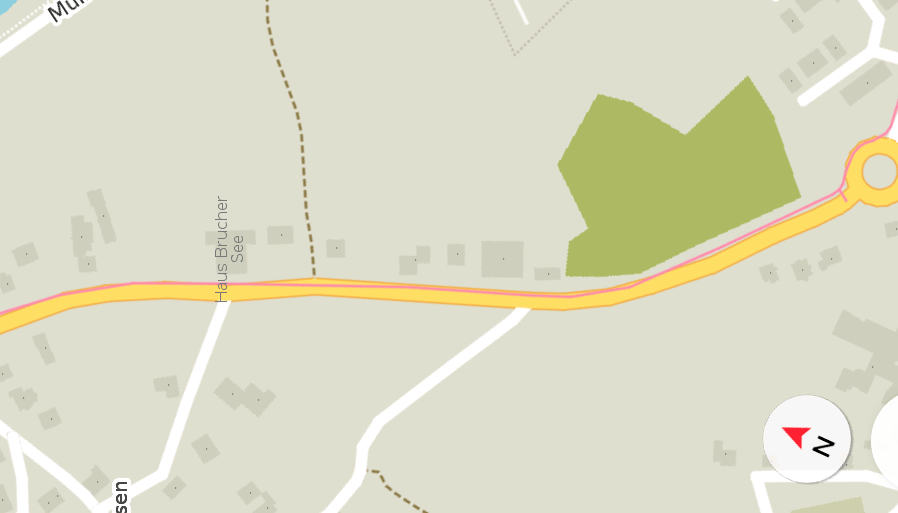
\includegraphics[width=\ScaleIfNeeded]{../chapter2/stuelinghausen-me}
	\caption
		[straßenbegleitender Radweg schneidet Straßenfläche]
		{straßenbegleitender Radweg (rot) schneidet Straßenfläche \citex[rotiert]{map:me}}
	\label{fig:stuelinghausen-maps.me}
	% Section 4 of the Apache License 2.0 used by maps.me permits relicensing of Derivative Works under different terms. It's not clear if this screenshot even qualifies as a Derivative Works under § 51 UrhG, but even if it does, relicensing under CC terms would be allowed as per the Apache License's terms.
}{
	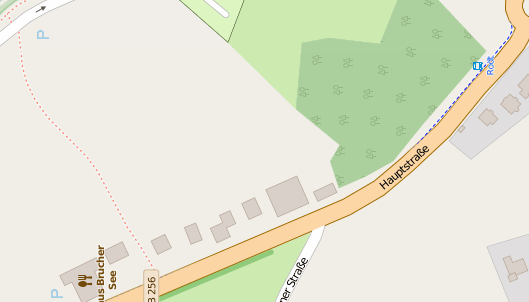
\includegraphics[width=\ScaleIfNeeded]{../chapter2/stuelinghausen@2-z17}
	\caption
		[straßenbegleitender Radweg von Straße verdeckt]
		{straßenbegleitender Radweg (blau strichliert) von Straße verdeckt \citex[rotiert]{map:osm-carto}}
	\label{fig:stuelinghausen-mapnik}
}

Abbildungen~\ref{fig:stuelinghausen-maps.me} und~\ref{fig:stuelinghausen-mapnik} zeigen beispielhaft, wie ein straßenbegleitender Radweg mal „über“, mal „unter“ der Straße zu liegen kommt.
Keiner dieser beiden Ansätze ist kartographisch gelungen.
Bevor eine Generalisierung durch Verdrängung stattfinden kann, muss zunächst der Konflikt zwischen Straße und Radweg erkannt werden.
Es ist denkbar, dass dies durch Untersuchen auf Parallelität geschehen oder erleichtert werden könnte.



\subsection{Generalisierung durch Zusammenfassung}

Die Generalisierung durch Zusammenfassung von Linienzügen kommt vor allem bei Parallelität in Betracht.
Dabei treten immer wieder in verschiedenen Situationen Darstellungsprobleme auf.

\label{dual-highway-case-2}

Beispielsweise variiert in OpenStreetMap auffallend oft der Abstand von zwei Richtungsfahrbahnen einer Straße.
Abbildung~\ref{fig:b256} zeigt, wie innerhalb weniger hundert Meter die Linearsignaturen zweier Richtungsfahrbahnen teilweise so weit voneinander entfernt liegen, dass dazwischen eine Lücke entsteht (Markierung~\textfiguremark{1}), aber teilweise auch so dicht beieinander, dass die Lücke geschlossen wird und die Randstriche der beiden Signaturen ineinander übergehen, was den Eindruck eines Mittelstriches wechselnder Strichstärke erwirkt (\textfiguremark{2}).
An einer Stelle sind die beiden Richtungsfahrbahnen gar so dicht beieinander gezeichnet, dass der Rand- bzw. Mittelstrich verschwindet und beide Fahrbahnen ineinander übergehen (\textfiguremark{3}).

\twofigures{ht}{
	\begin{overpic}[width=7cm]{../chapter2/b256@2-z16}
		\put(33,96){\figuremark[white]{1}}
		\put(96,81){\figuremark[white]{2}}
		\put(134,94){\figuremark[white]{3}}
	\end{overpic}
	\caption
		[variierende Abstände von Richtungsfahrbahnen]
		{variierende Abstände von Richtungsfahrbahnen \citex[bearbeitet]{map:osm-carto}}
	\label{fig:b256}
}{
	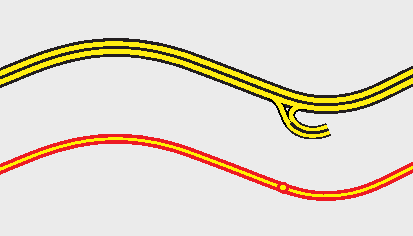
\includegraphics[width=\ScaleIfNeeded]{../chapter2/combined-symbols}
	\caption{kombinierte Signaturen für autobahnähnliche Straßen mit Anschlussstelle}
	\label{fig:dual-carriageway}
}

In Maßstabsbereichen, in denen die Grundrisstreue keine Rolle spielt, könnte möglicherweise eine stattdessen entlang der mittig zwischen den beiden Fahrbahnen verlaufenden Straßenachse gezeichnete kombinierte Signatur ein besseres Kartenbild erreichen (Abbildung~\ref{fig:dual-carriageway}).
Da jedoch in \osm\ die gesonderte Erfassung der Straßenachse unüblich ist, müssten hierzu zunächst die beiden Richtungsfahrbahnen als zusammengehörig (parallel) erkannt werden.

% TODO: evtl. Verweis auf ch2.1 / Sch09?
% siehe "Überleitung" unten!

% Grund für folgenden Absatz: zeigen, dass Verfahren von osm.de keine Lösung ist

In Deutschland erfasst die \osm-Community autobahnähnliche Straßen als \osmtag{highway}[trunk] anhand ihres Ausbauzustands.
Allerdings bildet die \osm-Straßenklassifizierung historisch bedingt das britische System ab, wo \term{trunk roads} ausdrücklich keinen bestimmten Ausbauzustand haben, sondern das Kernnetz der wichtigsten Straßen erster Ordnung bilden.
Unter Umständen wird \osmtag{highway}[trunk] somit auch für schmalere Landstraßen verwendet.

Wird den Gepflogenheiten in Deutschland entsprechend für \osmtag{highway}[trunk] eine auf den Ausbau mit baulich getrennten Fahrbahnen hindeutende Signatur gewählt, so birgt dies im internationalen Einsatz Potenzial für Verwirrung.
Abbildung~\ref{fig:trunk-norway-osm-de} zeigt eine solche Situation aus Norwegen:
Die Kartensignatur erweckt den Eindruck eines autobahnähnlichen Ausbaus, tatsächlich handelt es sich jedoch um eine einfache Landstraße mit Grundstückszufahrten und engen Kurvenradien (Abbildung~\ref{fig:trunk-norway}).

% TODO: Relationen-Probleme erläutern? -> eher weiter vorne!

% alternative Beispiele für schmale trunks in NO:
% Ev39 Kalandseidet, > 6 m aber Karte zeigt "mitten im Dorf"
% Ev39 Søfteland, Bild noch besser, aber keine Häuser in Karte
% Ev39 nach Nesttun rein, ginge auch, aber mit Radweg
%   https://goo.gl/maps/jYRgZVXft912
% Ev39 Vallaheiene wohl das beste hier
%   https://goo.gl/maps/wMHPCocqsSH2
% Rv13 Låtefossen, würde auch ohne Häuser in Karte funktionieren, < 6 m
% oder so Serpentinen, z. B. Granvin, gutes Bild aber keine Bebauung in Karte
%   https://goo.gl/maps/Y4NwWfRWSZ82

\twofigures{ht}{
	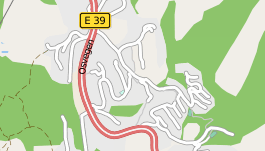
\includegraphics[width=\ScaleIfNeeded]{../chapter2/trunk-no-ev39-map1}
	\caption
		[Landstraße als {\osmtag{highway}[trunk]} mit autobahnähnlicher Signatur]
		{Landstraße (Vallaheiane) als {\osmtag{highway}[trunk]} mit \mbox{autobahnähnlicher} Signatur \citex{map:osm-de}}
	\label{fig:trunk-norway-osm-de}
}{
	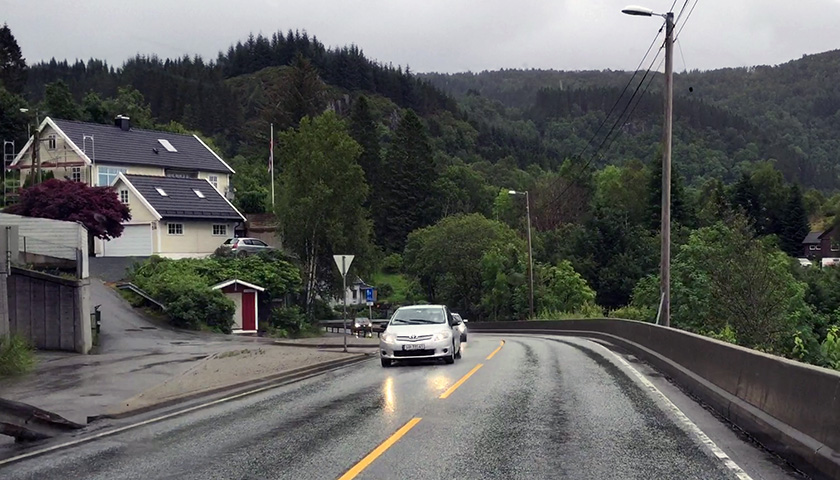
\includegraphics[width=\ScaleIfNeeded]{../chapter2/trunk-no-ev39-frame1639}
	\caption
		[typische norwegische Fernstraße \term{(riksveg),} als {\osmtag{highway}[trunk]} erfasst]
		{typische norwegische Fern\-straße (\term{riksveg} E\,39, Vallaheiane), als {\osmtag{highway}[trunk]} erfasst}
	\label{fig:trunk-norway}
}

Dass aus dem \osm-Datenmodell samt Attributen der tatsächliche Ausbauzustand oft nicht unmittelbar hervorgeht, macht die Möglichkeit einer algorithmischen Ableitung desselben aus der Geometrie der Geodaten interessant.
Möchte man einheitliche Zeichenregeln verwenden, so wäre auch hier die Möglichkeit einer Erkennung von zwei Richtungsfahrbahnen als parallel und zusammengehörig hilfreich.


% --------------------

% zu tracks=* - Überleitung evtl:
% Folge der oben beschriebenen offenen Arbeitsweise von \osm ist, dass das Herstellen einer Einigung über bestimmte Tagging-Varianten und deren Anwendung durch die Community oft ein langsamer Prozess ist. \noref[Sch09, forum 485926 s.u.]
% https://forum.openstreetmap.org/viewtopic.php?pid=485926

\label{railway-case}

Die Probleme durch fehlende Generalisierung durch Zusammenfassung sind nicht auf das Straßennetz beschränkt.
So wird in \osm\ mit \osmtag{tracks}[*] die Anzahl der Eisenbahngleise gekennzeichnet, für die ein \term{way} steht.
Die Karten in Abbildung~\ref{fig:tracks} stellen diesen \term{tag} farblich dar.

Bei Betrachtung in kleinem Maßstab sieht darin \textfiguremark{1} zunächst nach einer viergleisigen Strecke aus, in großem Maßstab plötzlich nach wenigstens \emph{zwei} viergleisigen Strecken nebeneinander.
Tatsächlich liegen insgesamt vier einzelne Gleise, die jeweils durch einen \term{way} mit dem Attribut \osmtag{tracks}[4] erfasst sind%
\footnote{Das \osmtag{tracks}-Attribut wurde zwischenzeitlich durch Beitragende von diesen \term{ways} entfernt.}.
In kleinem Maßstab fließen sie zusammen, in großem Maßstab sind sie jedoch einzeln erkennbar und vermitteln dem Leser das falsche Bild von insgesamt 16~Gleisen.
Möglicherweise hat ein \osm-Beitragender \osmtag{tracks}[*] missverstanden als die Gesamtanzahl der Gleise, \cf{Fox12} wofür jedoch das Attribut \osmtag{passenger\_lines}[*] zu verwenden ist.

\onedoublefigure{ht}{
	\begin{overpic}[width=\ScaleIfNeeded]{../chapter2/tracks-small}
		\put(92,63){\figuremark[white]{1}}
		\put(103,72){\figuremark[white]{2}}
		\put(95,13){\figuremark[white]{3}}
		\put(122,14){\figuremark[white]{4}}
	\end{overpic}
}{
	\begin{overpic}[width=\ScaleIfNeeded]{../chapter2/tracks-large}
		\put(33,75){\figuremark[white]{1}}
		\put(114,93){\figuremark[white]{2}}
		\put(76,10){\figuremark[white]{3}}
		\put(116,10){\figuremark[white]{4}}
	\end{overpic}
}{
	% fiktives Beispiel
	\caption
		[fehlerhafte Repräsentation der Gesamtzahl paraleller Gleise mit dem \osmtag{tracks}-Attribut]
		{fehlerhafte Repräsentation der Gesamtzahl paraleller Gleise mit dem \osmtag{tracks}-Attribut (links Zoom~15, rechts Zoom~17; Karlsruhe-Weiherfeld) \cf{map:ito-tracks}}
	\label{fig:tracks}
}

Analog kann in kleinem Maßstab der Eindruck entstehen, dass von der eingleisigen Strecke \textfiguremark{2} zwei doppelgleisige Strecken \textfiguremark{3} und \textfiguremark{4} derart abzweigen, dass am unteren Kartenrand insgesamt fünf Gleise nebeneinander liegen.
In größerem Maßstab wird erkennbar, dass es sich gerade umgekehrt verhält:
Die Strecke \textfiguremark{2} ist korrekt mit zwei parallelen Gleisen erfasst, deren Signaturen jedoch im kleineren Maßstab zusammenfließen;
die Abzweige \textfiguremark{3} und \textfiguremark{4} bestehen allerdings aus jeweils nur einem einzelnen Gleis, das fälschlich das Attribut \osmtag{tracks}[2] trägt.

% Fußnote?
Insgesamt sind die Darstellungen von \osmtag{tracks}[*] in Abbildung~\ref{fig:tracks} wenig gelungen%
\footnote{Hier zeigt sich eine Schwäche von \osm: Zwar ist mit \term{relations} eine logische Verknüpfung paralleler Gleise in der \osm-Datenbank technisch möglich, jedoch ist dies nicht zuverlässig und simpel genug, dass es von einer Mehrheit der \osm-Beitragenden angewandt wird.}.
Das unglücklich benannte Attribut \osmtag{passenger\_lines} reicht dazu aus, \osmtag{tracks}[*] für manche Anwendungen zu ersetzen, wird jedoch nur auf speziellen Karten angezeigt,
% zu implizit?
so dass es nicht annähernd flächendeckend erfasst ist (Abbildung~\ref{fig:passenger_lines}).

\onefigure{ht}{
	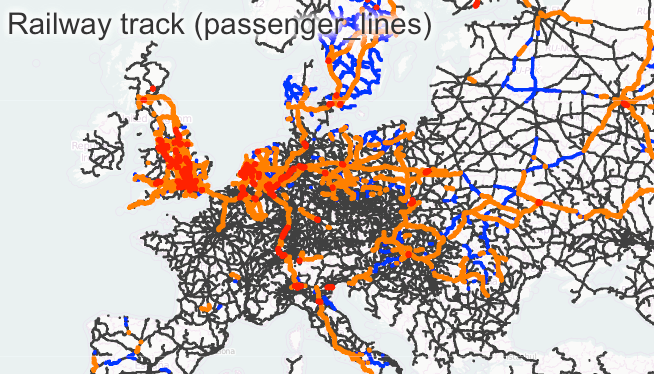
\includegraphics[width=\ScaleIfNeeded]{../chapter2/passenger_lines-europe}
	\caption
		[Eisenbahnstrecken in Europa, für die {\osmtag{passenger\_lines}[*]} erfasst ist]
		{Eisenbahnstrecken in Europa, für die \osmtag{passenger\_lines}[*] erfasst ist \citex{map:ito-passenger-lines}}
	\label{fig:passenger_lines}
}



%\subsection{Generalisierung durch Qualitätsumschlag}

%Beispiele für Qualitätsumschläge in Web-Karten sind schwierig zu finden. Oft handelt es sich bei entsprechenden graphischen Effekten technisch um eine Generalisierung durch Auswahl, durch die ein bisher verdecktes Element zum Vorschein kommt.



%\item Erkennung als parallel ist bisher ein Problem

\section{Zielsetzung der Arbeit}

Das automatisierte Zusammenfassen paralleler Linienzüge kann zur Vermeidung einiger der oben diskutierten Probleme bei der Generalisierung und Darstellung von Geodaten beitragen.

Bereits das Zusammenfassen selbst ist ein Vorgang der kartographischen Generalisierung.
Es kann das Kartenbild vereinfachen und verbessern.
% TODO: Abgleich mit oben

Beim Zusammenfassen könnten Attribute der beteiligten \term{ways} derart aggregiert werden, dass zuvor durch Geometrie ausgedrückte Zusammenhänge in den generalisierten Daten erhalten bleiben.
Beispielsweise könnte beim Zusammenfassen paralleler Gleise die in \osmtag{passenger\_lines} vermerkte Gleisanzahl der zuvor getrennten \term{ways} für das generalisierte Ergebnis addiert werden (vgl. Abschnitt~\ref{railway-case}).
Die so vereinfachten Geodaten können dann entsprechend ihrer Attribute visualisiert werden.
Die Gefahr von missverständlichen oder unschönen Kartenbildern, die wie oben gezeigt etwa durch Überlagerung entstehen können, wird so verringert.

Ebenfalls verringert wird die Datenmenge an sich.
Das Arbeiten mit Geodaten für große Gebiete, aber auch die Weiternutzung für andere Zwecke wird so unter Umständen einfacher.

Zum Beispiel sind automatisierte Formvereinfachungen einfacher durchzuführen, wenn keine Rücksicht auf eventuell parallele Linienzüge mehr genommen werden muss (siehe Abbildung~\ref{fig:crossing-parallels}).
% TODO: Referenz
% Zusammenfassung kann theoretisch auch Erstellen von MRDBs vereinfachen

Ziel \emph{dieser} Arbeit ist die Entwicklung von Algorithmen zur Generalisierung durch Zusammenfassung parallel verlaufender Linienzüge in \osm{}.
Weitere Generalisierungsvorgänge sind nicht Teil dieser Arbeit, insbesondere weder eine Formvereinfachung noch eine Verdrängung.



\section[Diskussion existierender Ansätze]{Diskussion existierender Ansätze zur automatisierten Linien-Generalisierung}
\label{ch:existing-approaches}

\subsection{Linien zusammenfassen mit Puffer}
\label{ch:buffer}
% - für eine Darstellung von OSM-Daten als Teil eines 3D-Modells werden Straßen "realistisch" verbreitert per Buffer in PostGIS
% - um Fragmente und Parallelen zu beseitigen, werden die so entstandenen Polygone nun vereinigt
% => Parallelen finden durch Buffer-Algorithmus und Polygonanalyse
% => Epsilon benötigt
% - Buffer orthogonal zur Linie würde reichen; die Endrundungen können wegfallen
% - löst Zusammenfassung nicht, da keine unmittelbare Rückführung zur Linie allein mit diesem Ansatz möglich (was für das erklärte Ziel 3D aber eh nix ausmacht, insofern ist der Ansatz gut, aber eben nicht gut für mich); evtl. inward offset (um wieviel?) oder eher -> Skeleton
% - löst auch Erkennung nicht

Das Projekt „OSM-3D“ verwendet \osm-Daten automatisiert zum Aufbau eines 3D-Modells für die ganze Welt.
Die \term{ways} aus \osm\ werden für die 3D-Szene durch Pufferung mit attributabhängigem Radius in Polygone gewandelt, um ein Gesamtbild mit realistischen Breiten von Straßen, Wegen und Bahnlinien zu erzeugen.
Um dabei durch Überlappungen von eng parallelen \term{ways} entstehende unnötig große Datenmengen zu vermeiden, werden diese Polygone anschließend vereinigt. \cf[2–3]{OHSZ10}

Durch diesen Ansatz werden unerwünschte Parallelen beseitigt.
Allerdings ist die für diese Arbeit erwünschte Rückführung des durch das Puffern entstandenden Flächen zu einer Linie nicht ohne Weiteres möglich.
Auch werden Parallelen nicht als solche erkannt, sondern entfallen restlos durch die Polygonvereinigung.
Daher erscheint dieser Ansatz isoliert betrachtet für die dieser Arbeit zugrundeliegende Fragestellung nicht geeignet.


\subsection{Bildung von Skelettlinien}
\label{ch:skeleton}
% - "In geometry, a straight skeleton is a method of representing a polygon by a topological skeleton." (<- Wikipedia)

Eine Möglichkeit, Flächen auf innere Linien zu reduzieren, bietet die Skelettierung.
Für das Straight Skeleton werden Polygone so lange sukzessive geometrisch verkleinert, bis nur noch ein aus geraden Linien zusammengesetztes topologisches Skelett übrig bleibt (Abbildung~\ref{fig:skeleton}).
Hierfür existieren unterschiedliche Algorithmen. \cf{wp:StraightSkeleton}

\onefigure{h}{
	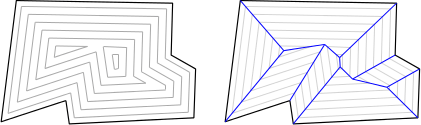
\includegraphics[width=\ScaleIfNeeded]{../chapter2/approach-skeleton}
	\caption
		[sukzessive Verkleinerung einer Fläche und deren Skelettlinien]
		{sukzessive Verkleinerung einer Fläche (links) und deren Skelettlinien (blau; rechts) \citex{Hub12}}
	\label{fig:skeleton}
}

% HS04: straight skeleton for MRDB
% <http://web.archive.org/web/20070613154012/http://www.ikg.uni-hannover.de/skalen/buendel/PDF/Skeleton.pdf>
% - Ziel: Framework für MRDB (automatisch)
% - erwähnt Chordal Axis (Prasad, 1997) ********
% - verwendet straight skeleton plus eine handvoll Regeln, um Kreuzungen etc. zu behandeln; immer noch etwas verwurstet, aber sieht wesentlich besser/systematischer aus als LM96
% - schlägt angeblich fehl an komplizierteren Stellen
% - ermittelt eine Relation zwischen ALK ATKIS

Haunert und Sester nutzen ein Straight Skeleton, um aus Flächen in der Automatisierten Liegenschaftskarte (ALK) Linien zur Nutzung in einer Multiple Representation Database (MRDB) abzuleiten.
Der Algorithmus von Eppstein und Erickson \citex{EE99} musste für die ALK-Daten angepasst und erweitert werden, um das resultierende Netz auf die gewünschten Mittellinien der Flächen zu reduzieren.
Dennoch kommt es zu teils erheblichen Problemen an Kreuzungen, die nicht in allen Fällen gelöst werden können. \cf[4–6]{HS04}

% Mig12: Projekt für "schöne" topo. Karte
% <http://mike.teczno.com/notes/osm-us-terrain-layer/foreground.html>
% <http://mike.teczno.com/img/terrain-stamen-post/> *******
% - erwähnt kurz Probleme von dual carriageways
% - eines der Probleme: unschöne versetzte Doppelungen von Straßennamen
% - Anwendung von Skeletron (mit Implementierung von LM96 für OSM)
% - Ziel letztlich "nur" Shields und Straßennamen

Migurski setzt eine Skelettierung ein, um für eine topographische Karte auf \osm-Basis Straßennamen und -nummern graphisch ansprechend darzustellen.
Im Falle von zwei zueinander parallelen Fahrbahnen derselben Straße sollen Nummer und Name so gezeichnet werden, dass sie für beide Fahrbahnen gelten und unschöne Doppelungen des Namens vermieden werden.
Hierzu benutzt Migurski die Software Skeletron. \citetext{\citealp{ME11}, cf. \citealp{Mig12}}

% Skeletron [ME11]:
% <https://github.com/migurski/Skeletron>
% - jetzt LM96, davor HS04 (?) "straight skeleton", was nicht so toll war

Skeletron benutzte ursprünglich ein Straight Skeleton nach dem erwähnten Ansatz von Haunert und Sester, was aber letztlich nicht besonders gut funktioniert hat („ultimately didn't work very well“ \citex[Readme]{ME11}).
Inzwischen wird die von Ladak und Martinez für diesen Zweck beschriebene Thiessen-Polygon-Methode eingesetzt.

% LM96: Straßen_flächen_ -> Einzellinie
% - Ziel: Eliminierung _oder_ Minimierung manueller Eingriffe
% - gute Ausgangsdaten seien entscheidend fürs Projekt gewesen (1:1000, mit Straßenflächen!)
% - ways werden verdichtet auf einen node alle 30 cm, um eine gesmoothte Mittellinie zu erhalten
% - ausgehend von nodes wird ein Voronoi-Diagramm gebaut, aus dem sich direkt die Mittellinie ergibt (nach filtern)
% - erzeugt schwierig zu filternde Dangles / Forks dort, wo Parallelen enden; Auflösung durch zusätzliche Angaben aus der Datenquelle ('The "true end" of the road is determined by temporarily appending the appropriate road extent arcs from the original Urban layer.')
% - "Suspect situations" kommen vor und werden manuell beseitigt
% - 7 man-months

Hierbei werden ausgehend von einer sehr detaillierten Straßenfläche zunächst deren Kanten verdichtet auf mehrere Knoten pro Meter, bevor ausgehend von diesen Knoten mittels Delaunay-Triangulierung ein Voronoi-Diagramm berechnet wird, dessen Kanten die Skelettlinien der Straßenfläche sind.
Auch hier ergeben sich allerdings erhebliche Probleme an allen Kreuzungen, die trotz Einbeziehung von Metadaten nur teilweise automatisch gefiltert werden.
Solche Fälle können immerhin automatisch erkannt und dann manuell beseitigt werden.
Der Aufwand für die Implementierung wird mit sieben Mann-Monaten beschrieben. \cf{LM96}

Um aus den \osm-\term{ways} Flächen zu erhalten, mit denen das Anwenden der Thiessen-Polygon-Methode erst möglich wird, puffert Skeletron zuvor die \osm-\term{ways} wie in Abschnitt~\ref{ch:buffer} beschrieben. \cf{ME11}


\subsection{Konflikterkennung}
\label{ch:conflict-detection}

%\item Conflict Detection \cf{KP98} \cf{Tho06a}
% KP98:
% - Ziel: gesamtes Straßennetz
% - detektiert Fälle, in denen Linien einander zu nahe kommen (wobei Bereiche nahe der Endknoten jeweils ausgeschlossen werden)
% - nutzt Voronoi region
% - eigentlich nicht speziell für parallelen gedacht oder geeignet (nutzt Dijkstra, um längeren von zwei Wegen zu eliminieren), aber speziell der "Second step: eliminate conflicts" könnte anwendbar sein, und der Voronoi-Kram gibt zumindest ein paar hübsche Bilder

Von Kreveld und Peschier beschreiben eine Möglichkeit, bei der automatischen Ableitung von Straßenkarten Konflikte nahe beieinander liegender Straßen zu erkennen und durch Auswahl nur einer der beteiligten Straßen aufzulösen.
Neben anderen Bedingungen werden so auch graphische Mindestabstände eingehalten. \cf{KP98}

Es liegt auf der Hand, dass sich parallele Straßen meist durch ein Unterschreiten dieser Mindestabstände auf ihrer gesamten Länge auszeichnen.
Das beschriebene Verfahren untersucht allerdings lediglich den minimalen Abstand zweier Straßen.
Das Untersuchen der gesamten Länge der Straße wäre erheblich teurer. \cf[4.]{KP98}
Dieser Ansatz erscheint daher für diese Arbeit wenig erfolgversprechend.

% Tho06a: ? Bib, einzelne Fotos in "neu"
% - erwähnt ausdrücklich mein Problem als "hilfreich" (in gelöstem Zustand)
% - Skeleton??

Thom erwähnt ausdrücklich, dass die Erkennung eines Konflikts von parallelen Straßenabschnitten für die automatische Generalisierung hilfreich wäre („... recognizing stretches of parallel road sections would help their automatic generalization“ \citex[676]{Tho06a}), allerdings ohne dabei eine mögliche Lösung anzudeuten.


%\subsection{Kognitive Wahrnehmung}
\subsection{Visuelle Wahrnehmung}

% Tho06b: Netzwerk-Generalisierung und -Analyse
% - perzeptueller Ansatz zur Defragmentierung und Auswahl-Generalisierung
% - primär Behandlung kollinearer Linien, erwähnt beiläufig aber auch Erkennung von Parallelen [evtl. mehr in den zahlreichen Referenzen darin?]
% - "perceptual grouping" [684]

Thomson beschreibt, wie das menschliche Gehirn optisch wahrgenommene Elemente selbst dann „spontan organisiert“, wenn deren Semantik völlig unbekannt ist.
Er bezeichnet dieses Konzept als „perceptual grouping“ und zählt unter den dazu herangezogenen geometrischen Eigenschaften neben Nähe, Ähnlichkeit und Symmetrie auch Parallelität und Kontinuität auf. \cf[683–684]{Tho06b}

% EM00:
% - erwähnt sehr deutlich meine Probleme mit "hanging streets" an Kreuzungen etc. [3]
% - erwähnt keine Parallelen, zeigt aber Implementierung der Theorien von Tho06b bzw. TR99

Zusammen mit Richardson beschreibt er eine Möglichkeit, die Eigenschaft der Kontinuität von Linienzügen (genannt \term{stroke}) zu nutzen, um deren Wichtigkeit einzustufen und damit ein Straßennetz zu generalisieren („Principle of Good Continuation“, Abbildung~\ref{fig:strokes}). \cf{TR99}
Edwardes und Mackaness nutzen denselben Ansatz zur Analyse des Netzes, um damit ihre auf Graphentheorie basierende Generalisierung zu unterstützen. \cf{EM00a}
Wie ein „perceptual grouping“ nach der Eigenschaft der Parallelität aussehen könnte, wurde nach Kenntnis des Verfassers bisher nicht konkret untersucht.

\onefigure{h}{
	\includegraphics[width=\ScaleIfNeeded]{../chapter2/approach-strokes_51}
	% copyrighted image used under § 51 UrhG - not included in git repository
	\caption
		[ein Netzwerk und seine \term{strokes} {[\copyright]}]
		{ein Netzwerk (a) und seine \term{strokes} (b) \citex[\term{figure} 2][\copyright]{TR99}}
	\label{fig:strokes}
}

% ! OS MasterMap
% CM05: ganzheitlicher Ansatz für Ordnance Survey in Road Network
% - arbeitet primär mit Strokes; Problem dabei: "good continuation" sieht an Gabelungen u. U. je nach Seite unterschiedlich aus; zur Lösung werden Attribute herangezogen
% - Fig 10 zeigt Resultat, welches Parallelen hat, welche nicht erwähnt werden
% - hebt Kreuzungsproblem als ungelöst hervor

Chaudry und Mackaness schlagen das Konzept von \term{strokes} zur Generalisierung von Straßennetzen durch Auswahl wichtiger Straßen für die digitale OS~MasterMap des Ordnance Survey vor.
Sie betonen jedoch, dass trotz ermutigender Resultate noch weitere Probleme gelöst werden müssen.
Auf die Eigenschaft der Parallelität gehen sie nicht ein. \cf{CM05}

% (ähnelt grob meinem Ansatz)
% Tho05: speziell meine Problemstellung!
% - Ziel: Hilfe bei automatischer Folgekartenableitung beim Ordnance Survey
% - 3 wichtigste Teile: Kreuzungsproblem, Verdrängung und Zusammenfassung von Parallelen [2]
% - arbeitet mit Strokes basierend auf one-way-Attributen; Probleme an manchen Kreuzungen, die aber automatisch erkannt und behoben werden sollen
% - Paarbildung erfolgt abhängig von Klassifizierung der Strokes (z. B. bei Verkehrsinseln kleinere Höchstschwelle als bei normalen Straßen)
% - Ausgangsdaten sind klassifiziert nach "dual carriageway" oder nicht (DESHALB nicht 1:1 auf OSM anwendbar, denn es gibt keinen solchen tag)
% - klappt nicht in allen Fällen (einzelne Fehlerfälle)
% - benutzt Skeleton zur tatsächlichen Zusammenfassung der erkannten Paare
% - funktioniert meistens, aber nicht immer; manche der Restfälle manuell als nicht lösbar erkannt
% - one-way-Attribut war "essential"
% - Ergebnis hat noch keine Topologie (future work)
% - erst mit Topologie ist Unterbrechung der Signatur möglich, um Ampelkreuzungen im Dual Carriageway darzustellen
% - Kreisverkehre werden bisher ignoriert

\label{os-mastermap}

Thom beschreibt vier Schritte zum Zusammenfassen getrennter Richtungsfahrbahnen von zweibahnigen Straßen und Verkehrsinseln auf eine gemeinsame Mittellinie für die OS~MasterMap.
Zunächst werden unter Nutzung von \term{strokes} und Attributen durchgehende Linienzüge für die Gesamtlänge der getrennten Richtungsfahrbahnen erzeugt, die dann durch Graphenanalyse ihrer jeweiligen Enden einander zugeordnet werden können.
Anschließend kann durch Skelettierung die Mittellinie der zugeordneten Linienzüge berechnet und im letzten Schritt noch Korrekturen an deren Enden vorgenommen werden. \cf[3–10]{Tho05}

Diese Schritte liefern in vielen Fällen ein gutes Ergebnis, was Thom der Attributierung der Ausgangsdaten zuschreibt.
Entscheidend ist insbesondere das „one~way“–Attribut sowie die Klassifikation nach Bauart der Straße (einbahnig, zweibahnig, Verkehrsinsel, Kreisverkehr etc.). \cf[14]{Tho05}


\subsection{Graphenanalyse}
\label{ch:graph-based}

% TR95: Graphentheorie in der Generalisierung von Straßennetzen
% - betont, dass autom. Generalisierung oft Darstellungs-zentriert ist und Topologie des Ergebnisses vernachlässigt [1871]

% MB93: Graphentheorie in der Generalisierung allgemein
% - durch Prüfung der Einbahn-Richtung erkennen, ob insgesamt ein verbundener Graph vorliegt (zweimal Einbahn => einmal Zweibahn)
%\cf{MB93}

Frühe Entwicklungen der automatisierten Generalisierung versuchten oft, unter Vernachlässigung der Topologie des Ergebnisses den Fokus des Kartographen auf der Visualisierung nachzuahmen. \cf[1871]{TR95}
Ansätze der Graphentheorie können jedoch nicht nur wie zuvor beschrieben andere Methoden unterstützen, sondern auch direkt zur Generalisierung eingesetzt werden.

% HAS05: will typische Muster erkennen
% - erwähnt für Strokes Problem dort, wo Richtungsfahrbahnen beginnen, mitsamt theoretischer Lösung [3.2]
% - evtl. können Parallelen in einem Netzwerk durch Musteranalyse erkannt werden (typischerweise sehr lang und schmal); jedoch vmtl. Probleme an Kreuzungen etc.

Heinzle et~al. zeigen Methoden, um typische Muster in Straßennetzen zu erkennen und daraus Informationen abzuleiten. 
Es liegt auf der Hand, dass parallele Fahrbahnen einer zweibahnigen Straße ein typisches Muster sein können, jedoch werden diese nur beiläufig erwähnt. \cf[3.2.]{HAS05}

% JC04: connectivity graph für urban street network
% - dreht Straßen-Graph logisch um (Knoten=Straße, Kante=Verbindung)
% - filtert nach Graphkriterien ("centralities" degree, closeness, betweenness)
% - Ergebnis ist ein nach natürlich Kriterien modellgeneralisiertes Netz, denn Straßen mit besserer Verbindung werden häufiger benutzt und sind somit wichtiger
% - Parallelen im Straßennetz zeichnen sich durch Redundanz und Symmetrie aus (oft gegeneinander gerichtete Einbahnstraßen) und sind damit höchstens! in einem sehr unregelmäßigen Netz theoretisch! erkennbar; tatsächlich werden im Beispiel im Paper die Parallelen nicht generalisiert [168]

Jiang und Claramunt verwenden Zentralitätsmaße, um die wesentliche Struktur eines Straßennetzes zu identifizeren und bei der Generalisierung zu erhalten.
Dieser Ansatz entspricht dem Prinzip, dass schlechter ans Netz angebundene Straßen weniger wichtig sind als jene, die gut angebunden sind („less connected streets are less important than those well connected from a structural point of view“ \citex[161]{JC04}). \cf{JC04}
Für parallele Kanten im Graph ist allerdings zu erwarten, dass sie jeweils ähnlich gut an den Rest des Netzes angebunden sind, weswegen dieses Kriterium für diese Arbeit nicht als nützlich erscheint.

% MM99: Simplification of Junctions
% - "Brücken von Königsberg" als Beispiel für junction simplification und Zusammenfassung von Parallelen, aber das ist wohl etwas zu sehr vereinfacht! [188]
% - evtl. werden durch Zusammenfassen der Kreuzung von Parallelen jene zu Duplikaten und können so erkannt und zusammengefasst werden; Nachteil: klappt wirklich nicht ohne Kreuzungen (diese Methode wird anscheinend nicht explizit erwähnt)

Probleme an Kreuzungen wurden bereits von mehreren Autoren genannt.
Mackaness und Mackechnie demonstrieren eine Methode, um Straßenkreuzungen durch eine Kombination von räumlicher und graphentheoretischer Analyse zu identifizieren und zu vereinfachen. \cf{MM99}
Der Gedanke, dass etwa im Falle einer zweibahnigen innerstädtischen Straße durch Generalisierung komplexer Kreuzungen auf einen einzelnen Punkt die vormals nur geometrisch parallelen Kanten zu zwei topologisch parallelen Kanten (Mehrfachkanten) in einem ungerichteten Graphen des Straßennetzes werden, welche dann leicht zusammenzufassen sind, liegt im Kontext dieser Arbeit nahe.
Die Arbeit von Mackaness und Mackechnie berücksichtigt diesen Aspekt allerdings nicht.


%\begin{itemize}
%\item \cf{Kne09}
% Kne09: Anwendung von Graphentheorie in OSM, wenig hilfreich für uns
% ! Relational Constraints
%\item Relational Constraints \cf{TBDJRG12}
% - hat keinen Algorithmus, sondern nur Konzepte
% - führt constraint ontology ein als mögl. Hilfswerkzeug
% evtl. als Grundlage für Kap. 4 interessant
%\end{itemize}

% + RoadMatcher 
% <http://wiki.openstreetmap.org/wiki/Roadmatcher>
% + http://sourceforge.net/projects/jump-pilot/files/OpenJUMP_plugins/More%20Plugins/Matching%20PlugIn/
% <http://sourceforge.net/projects/jump-pilot/files/OpenJUMP_plugins/More%20Plugins/Matching%20PlugIn/>

%(jeweils einschließlich Anwendbarkeit auf die vorliegende Fragestellung, ggf. Vor- und Nachteilen, ggf. Bezug der darin verwendeten Fachsprache zur in dieser Arbeit verwendeten Terminologie)



% single-chapter commands
\onlyinsubfile{\listoffigures} %\onlyinsubfile{\listoftables}
%\onlyinsubfile{% UTF-8

\documentclass[../main/thesis.tex]{subfiles}
\begin{document}

% include works in bibliography that aren't cited anywhere in the document (for debugging)
\onlyinsubfile{\nocite{*}}


\defbibnote{thesisBibIntro}{\justify%
Die Literaturangaben sind alphabetisch nach dem Kürzel sortiert.
Das Kürzel wird gebildet aus den ersten drei Buchstaben des Nachnamens des Autors, bei mehreren Autoren aus jeweils den Anfangsbuchstaben der Nachnamen, bei Körperschaften aus einer mnemonisch gewählten Folge von Kleinbuchstaben; jeweils ergänzt durch die letzten beiden Ziffern des Jahres der Veröffentlichung.
\par
Um ein eventuelles Nachschlagen zu erleichtern, sind die Referenzen wo immer möglich durch Angabe von Orten ergänzt, an denen eine Kopie des jeweiligen Werks am 1.~März 2018
% gegen 22~Uhr
aufzufinden war.
In der PDF-Ausgabe dieses Dokuments sind die URLs Hyperlinks.
Die Signaturen beziehen sich auf die Bibliothek des Karlsruher Instituts für Technologie und deren Standort „Fachbibliothek HsKA“.
\bigskip}


\RaggedRight
\addtocontents{toc}{\medskip}
\newpage\addcontentsline{toc}{chapter}{Literaturverzeichnis}
\printbibliography[title=Literaturverzeichnis,prenote=thesisBibIntro]

\end{document}
}
\end{document}
